%%This is a very basic article template.
%%There is just one section and two subsections.
\documentclass{article}
\usepackage[utf8]{inputenc}
\usepackage{a4wide}
\usepackage{german, amsfonts, amssymb, amsmath, ulem, amsthm, amstext}
\usepackage{enumerate}
%\usepackage[latin1]{inputenc}
\usepackage{caption,graphicx,wrapfig}
\usepackage{gauss}
\setcounter{tocdepth}{4}   %= Aufnahme in das Inhaltsverzeichnis *
\setcounter{secnumdepth}{4}  % = Nummerierung vertiefen *
\usepackage{graphicx}

\newcommand{\dpP}{\partial \Phi}
\newcommand{\dpXi}{\partial \xi}
\newcommand{\dpEta}{\partial \eta}
\newcommand{\dpX}{\partial x}
\newcommand{\dpY}{\partial y}
\newcommand{\ddt}{\frac{\partial }{\partial t}}
\newcommand{\ddx}{\frac{\partial }{\partial x}}
\newcommand{\ddy}{\frac{\partial }{\partial y}}
% ä ö includen
% TODO am ende \mathbf vor jedes Phi
  
\begin{document}

\title{Pratkikumsbericht zur Vorlesung \\Numerische Strömungssimulation}
\author{Thomas Camminaidy (297538), Peter Collienne (296711)}
\date{\today}
\maketitle \newpage

\tableofcontents \newpage


\section{Einleitung}
Der Vorliegende Bericht fasst die Inhalte des Programmierpraktikums zur Vorlesung Numerische Strömungssimulation 
im Sommersemester 2012 bei Dr.-Ing. Bernd Binninger zusammen. Die
Programmieraufgaben lassen sich in vier Themen unterteilen die in diesem Bericht enthalten sind. Ziel des Praktikums war es einen eigenen Strömungslöser mit Gittergenierirung zu implementieren und anhand verschiedener Testfälle zu validieren.
Zuerst befassten wir uns mit der Potentialströmung und einem passenden Lösungsverfahren. Anschließend fertigten wir einen 
Gittergenerator an, den wir im nächsten Schritt als Grundlage für die Lösung der Konvektions-Diffusions-Gleichung 
und anschließend der Impulsgleichung verwendet haben.


\section{Potentialströmung}
Potentialströmungen beschreiben das Strömungsfeld unter der Annahme einer inkompressiblen, reibungsfreien, wirbelfreien, zweidimensionalen
Strömung. Die Geschwindigkeiten des Fluids ergeben sich dann als Ableitung der Potential- bzw. Stromfunktion.
\begin{align} u =\frac{ \partial \Phi} {\partial x} \text{ und } v =\frac{ \partial \Phi} {\partial y}\end{align}
Mit Hilfe dieser Beschreibung der Geschwindigkeiten und unter Anwendung der Kontinuitätsgleichung 
lässt sich dann die 
2D-Laplace Gleichung für die Potentialfunktion $\Phi$ beschreiben.
Ausgangspunkt für die Beschreibung der Strömung ist die Kontinuitätsgleichung, welche unter Berücksichtigung von (1) eine 2D-Laplace Gleichung für die 
Potentialfunktion $\Phi$ darstellt.
\begin{align} &\nabla \cdot \mathbf{v} =0 \\ \Leftrightarrow &\frac{ \partial u} {\partial x}+ \frac{ \partial v} {\partial y}=0
\\ \Leftrightarrow &\Delta \Phi = 0 \end{align}
Neben der Potentialfunktion erfüllt ebenfalls die Stromfunktion $\Psi$ eine Laplacegleichung. Charakteristisch für Potentialströmungen
ist, dass die Isolinien der Potentialfunktion und Stromfunktion Senkrecht aufeinander stehen. Dies wird im folgenden auch als Kriterium für die
Bewertung unserers Programms benutzt. Zusätzlich zu der Laplacegleichung benötigt eine PDE auch noch Randbedingungen die durch die gegebene Geometrie
und z.B. Haftbedingungen vorgegeben sind.


\subsection{Diskretisierung auf einem äquidistanten orthogonalen Gitter}
Um die Laplacegleichung (2) zu lösen müssen die Ableitungen numerisch mittels finite Differenzen Approximiert werden.
Auf einem äquidistanten lassen sich die Laplacegleichung $\Delta \Phi = 0$ schreiben als
\begin{align}
\frac{\Phi_{i+1,j}-2\Phi_{i,j}+\Phi_{i-1,j}}{\Delta x^2}+\frac{\Phi_{i,j+1}-2\Phi_{i,j}+\Phi_{i,j-1}}{\Delta y^2}=0
\end{align}
Dabei bezeichnet $i$ den Laufindex in x-Richtung, also $x_i = \Delta x \cdot i$ und $j$ analog den Laufindex in y-Richtung.
Um eine Iterationsvorschrift für $\Phi_{i,j}$ zu erhalten, wird Gleichung (5) umgeformt.
\begin{align}
\Phi_{i,j} =\frac{\Delta x^2(\Phi_{i,j+1}+\Phi_{i,j-1})+\Delta y ^2(\Phi_{i+1,j}+\Phi_{i-1,j}) }{2(\Delta x^2 + \Delta y^2)}
\end{align}
Um für die Potentialfunktion zu lösen, iterieren wir mit Vorschrift (6) solange über unser Rechengebiet, bis $\Phi$ auskonvergiert ist.
Das Jacobi- und das Gauß-Seidel-Verfahren sind zwei mögliche Implementierungen. Der Unterschied zwischen den beiden Methoden liegt 
in der Verwendung der benachbarten Gitterpunkte $\Phi_{i\pm1, j\pm1}$. Das Jacobi-Verfahren verwendet dabei die Punkte aus dem Letzten Iterationsschritt,
während das Gauß-Seidel-Verfahren schon im momentanen Zeitschritt aktualisierte Punkte berücksichtigt. Das Gauß-Seidel-Verfahren konvergiert dabei in 
unseren Testfällen deutlich schneller als das Jacobi-Verfahren. Als weitere Option der Konvergenzbeschleunigung lässt sich das Gauß-Seidel-Verfahren 
noch mit einem Relaxationsfaktor versehen, bei dem entweder eine Über- oder eine Unterrelaxation verwendet werden kann.

\subsubsection{Testfall Parallelströmung} 
Zu Beginn wählen wir uns einen möglichst einfachen Testfall. Dazu setzen wir $\Omega =[0,1]^2$ als Einheitsquadrat welches 
wir in 20 Punkte in X-Richtung und 20 Punkte in Y-Richtung aufteilen. Als Fehlertoleranz setzen wir $\epsilon= 1e-6$.
und setzen das Potential am linken Rand fest auf $\Phi = 2$ und für den rechten Rand $\Phi = 0$.
Die beiden Grafiken Zeigen die Isolinien der Potential- und Stromfunktion.\\
\includegraphics[scale=0.5]{test/1parallel/phi.eps} 
\includegraphics[scale=0.5]{test/1parallel/psi.eps}  \\
Die folgende Grafik legt die Isolinien von Psi und Phi übereinander. Es zeigt sich, dass diese wie
gefordert senkrecht aufeinander stehen.\\ 
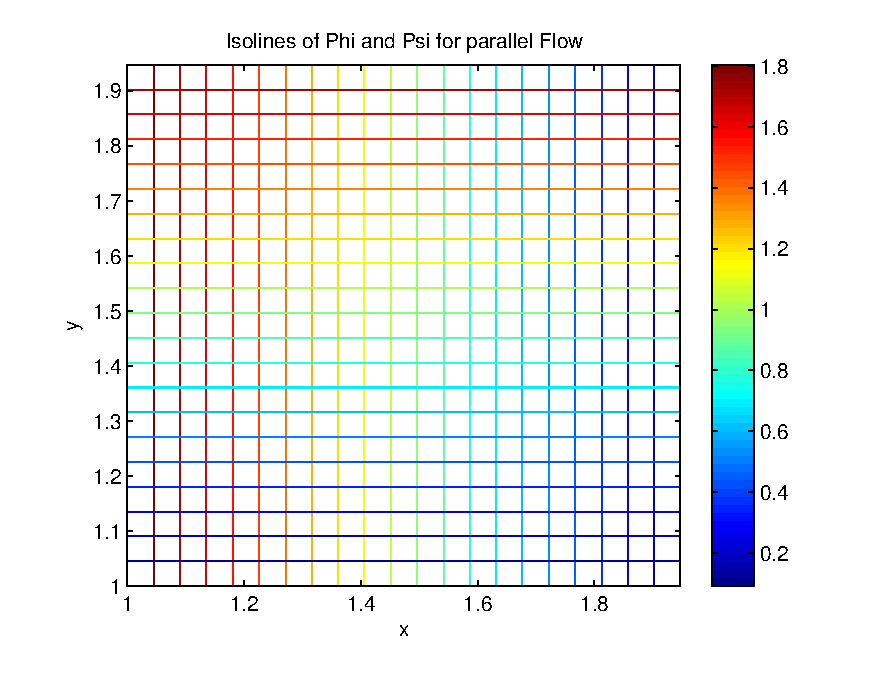
\includegraphics[scale=0.6]{test/1parallel/both.eps}\\
Das Gauß-Seidel-Verfahren konvergiert nach 1079 Schritten. Im nachstehenden Plot ist zu sehen, dass die Konvergenzgeschwindigkeit
mit zunehmender Iterationsanzahl zunimmt. Dieses Phänomen lässt sich an mehreren Testefällen vorfinden.\\
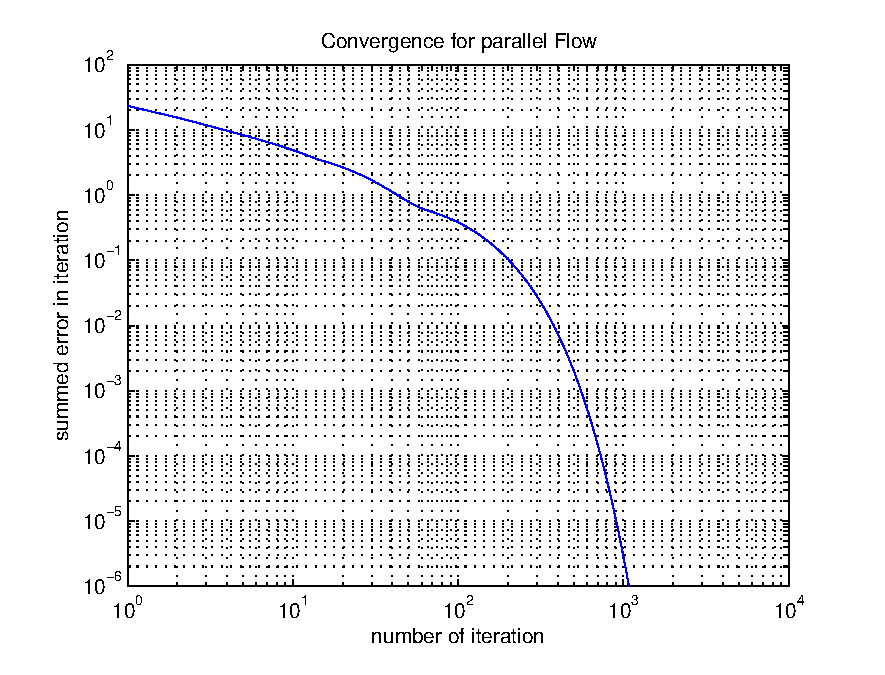
\includegraphics[scale=0.7]{test/1parallel/error.eps}

\subsubsection{Testfall Wirbel}
Als zweiten Testfall haben wir die Potentialfunktion für einen Wirbel gewählt.
Das Gebiet für diesen Fall ist $\Omega =[1,2]^2$ mit erneut 20 Punkten pro Dimension. 
Der Wirbelmittelpunkt befindet sich im Punkt
$(0,0)$. Das Potential für einen Wirbel ergibt sich zu
\begin{align}
\Phi = \frac{E}{2\pi}\arctan\Bigl(\frac{y}{x}\Bigr)
\end{align}
Analog ergibt sich die Stromfunktion zu
\begin{align}
\Psi = -\frac{E}{2\pi}\sqrt{{y}^2+{x}^2}
\end{align}
Der Wirbelmittelpunkt wurde bewusst außerhalb des Gebietes gewählt, da 
mit der obigen Iterationsorschrift für $\Phi$ nur endliche Werte erzeugt werden;
im Wirbelmittelpunkt hat das Potential allerdings eine Singularität. In unserem Fall
haben wir $\frac{E}{2\pi}=1$ gewählt.
Zu sehen sind erneut die Isolinien der Potential- und Stromfunktion.\\
\includegraphics[scale=0.4]{test/2vortex/phi.eps}
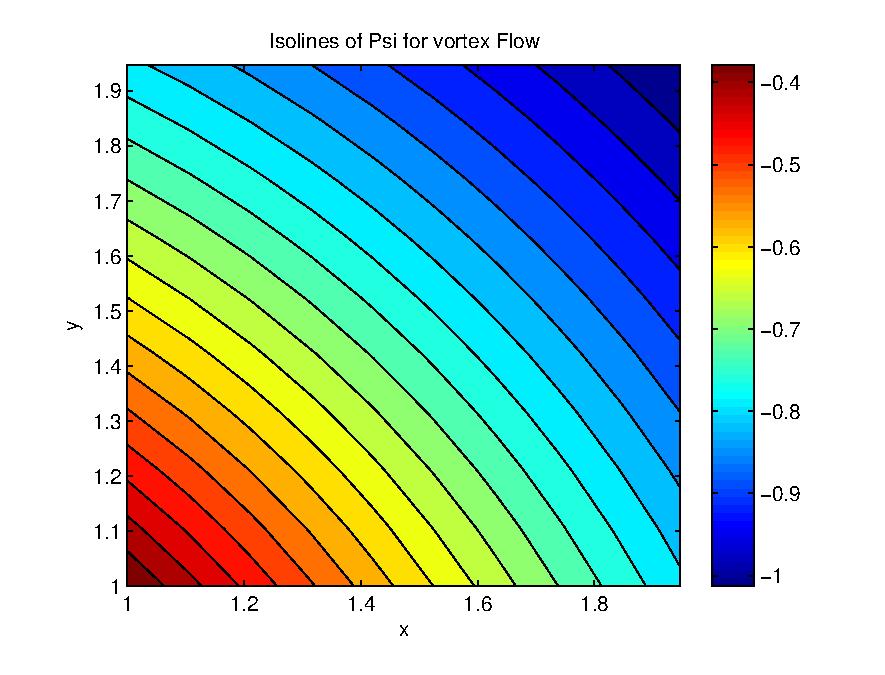
\includegraphics[scale=0.4]{test/2vortex/psi.eps}\newpage
Im folgenden sind die Isolinien überlagert. Es wird auch hier deutlich,
dass diese senkrecht aufeinander stehen.\\
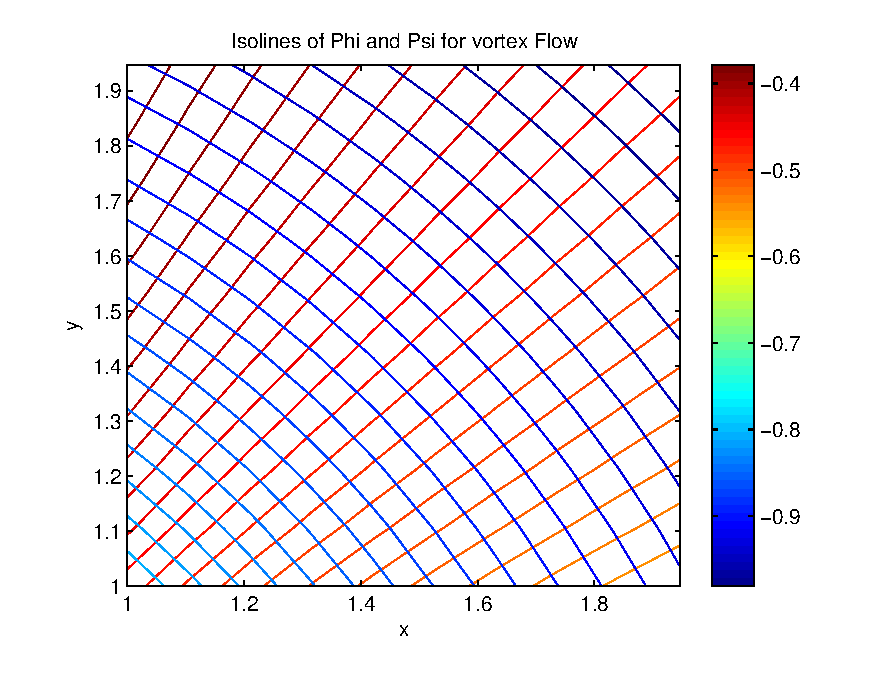
\includegraphics[scale=0.6]{test/2vortex/both.eps}\\
Die Relaxation erstellt in jedem Iterationsschritte die Lösung im Folgeschritt als Linearkombination aus der Lösung im letzten Schritt
und dem aktuellen Schritt.
\begin{align}
\Phi^{k} = \Phi^{k-1} + \beta (\Phi^{\tilde{k}}-\Phi^{k-1})
\end{align}
Für Die Iteration wurden unterschiedliche Werte für den Relaxationsfaktor gewählt. Dabei sieht man signifikante
Unterschiede in der Anzahl der benötigten Iterationsschritte.
So benötigt das Gauß-Seidel-Verfahren ohne Relaxation 601 Iterationsschritte um die Toleranz von $\epsilon= 1e-6$ 
zu erreichen. Wesentlich schneller konvergiert das Verfahren für $\beta = 1.8$. Zusätzlich sind noch die Fehlerplots
für $\beta = 0.9$, $\beta = 1.3$, $\beta = 1.9$ beigefügt.

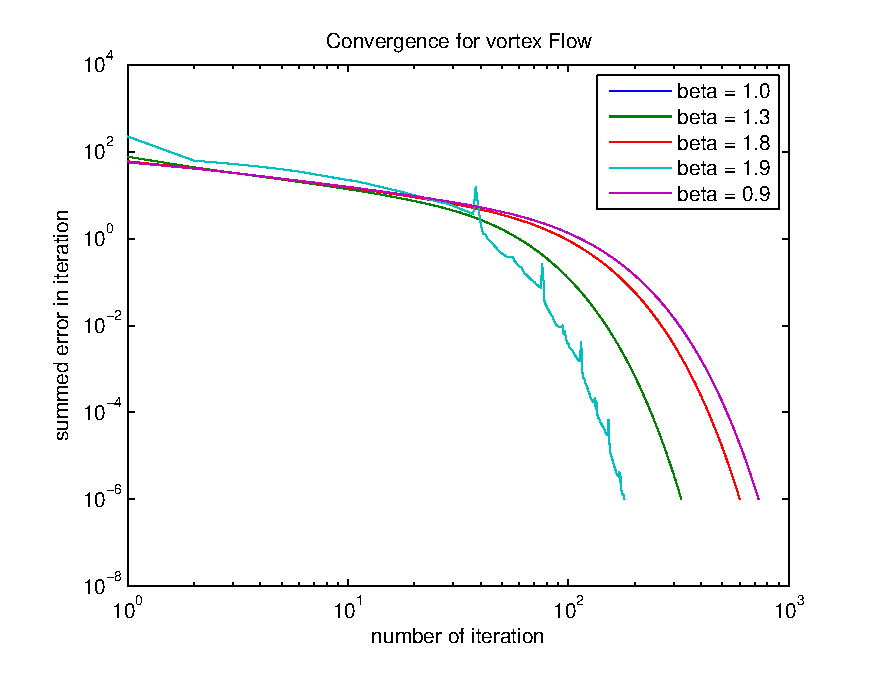
\includegraphics[scale=0.5]{test/2vortex/allerror.eps}


\subsection{Diskretisierung auf einem äquidistanten krummlinigen Gitter}
Da in der Realität die Geometrie der Objekte wesentlich komplexer ist, kommt es fast immer zu krummlinigen Integrationsgebieten.
Um die Laplacegleichung aber weiter wie gewohnt lösen zu können, versucht man, die physikalische Ebene auf ein rechteckiges Rechengebiet
zu transformieren. Dabei transformieren wir die Koordinaten von der $x-y-$Ebene in die $\xi-\eta-$Ebene des Rechengebietes. Wodurch sich folgende
Beziehungen ergeben
\begin{align}
&x = x(\xi,\eta) \ &y = y(\xi,\eta)\\
&\xi=\xi(x,y) \  &\eta=\eta(x,y)  
\end{align}
Durch diese Abhängigkeiten, ergeben sich beim Berechnen der 2. Ableitungen für die Laplacegleichung zusätzliche Terme,
resultierend aus der Kettenregel.
Somit transformiert man die Laplacegleichung zu
\begin{align}
\Bigl( \alpha_1 \frac{\partial^2}{\partial \xi^2} 
+\alpha_2 \frac{\partial^2}{\partial \eta^2} 
+\alpha_3\frac{\partial^2}{\partial \xi \partial \eta}
+\alpha_4 \frac{\partial}{\partial \xi} 
+\alpha_5 \frac{\partial}{\partial \eta} +\alpha_6 \Bigr ) \Phi=0
\end{align}
wobei $\alpha_{1},\ldots,\alpha_{6}$ aus den Ableitungen der Beziehungen in (7) und (8) und der gegebenen Geometrie
resultieren.
Dabei wird einfacheitshalber auf ein Rechengebiet transformiert für das $\Delta \xi=\Delta \eta=1$ gilt.
Somit ergibt sich analog zu (6) die Iterationsvorschrift für $\Phi_{i,j}$ auf einem krummlinigen Gitter zu
\begin{align}
8(\alpha_1+\alpha_2)\Phi_{i,j}  
&= \Phi_{i-1,j-1} \alpha_3 \\
&+\Phi_{i,j-1}(4\alpha_2-2\alpha_5) \notag \\
&-\Phi_{i+1,j-1} \alpha_3 \notag \\
&+\Phi_{i-1,j} (4\alpha_1-2\alpha_4)\notag  \\
&+\Phi_{i+1,j} (4\alpha_1+2\alpha_4)\notag  \\
&-\Phi_{i-1,j+1} \alpha_3\notag  \\
&+\Phi_{i,j+1} (4\alpha_2+2\alpha_5)\notag \\
&+\Phi_{i+1,j+1}\alpha_3 \notag 
\end{align}
\subsubsection{Randbedingungen}
\paragraph{Einström- und Ausströmränder}
$~~$\\
Als Randbedingungen für Ein- und Austrittsrand genügt ein einfaches Geschwindigkeitsprofil, dass durch Integration
in eine passende Randbedingung für die Potentialgleichung überführt werden kann.
In unseren Testfällen beschreiben wir das parallele Einströmen des Fluids in unsere Geometrie,
weshalb das Potential an Ein- und Austrittsrand jeweils konstant gesetzt wird.
\paragraph{Undurchlässige Wände}
$~~$\\
Auf dem Rand folgt die Strömung der Kontur, da die Potentialströmung eine reibungsfreie Strömung beschreibt.
Deshalb gilt auf dem Rand 
\begin{align}
\frac{dh}{dx} = \frac{v}{u} = \frac{\partial \Phi}{\partial y}\Bigl(\frac{\partial \Phi}{\partial x}\Bigr)^{-1}
\end{align}
Somit folgt für den transformierten Raum
\begin{align}
\frac{dh}{dx} = \Bigl(\frac{\dpP}{\dpEta}\frac{\dpEta}{\dpY}+ \frac{\dpP}{\dpEta}\frac{\dpEta}{\dpY}\Bigr)
\Bigl(\frac{\dpP}{\dpEta}\frac{\dpEta}{\dpX}+ \frac{\dpP}{\dpEta}\frac{\dpEta}{\dpX}\Bigr)^{-1}
\end{align}
Statt der Anwendung von zentralen finiten Differenzen muss am $\eta-$Rand auf die Formulierung mittels einseitiger finiter Differenzen
zurückgegriffen werden. Einsetzen der einseitigen Differenzen in $\eta-$Richtung in Gleichung (12) liefert eine Vorschrift zur Berechnung von
$\Phi_{0,j}$ bzw $\Phi_{N,j}$.
Die notwendige Ableitung $\frac{dh}{dx}$ wird auch mittels finiter Differenzen aus der vorgegebenen Kontur berechnet.
In der Implementierung wird dann in jedem Iterationsschritt zuerst $\Phi_{0,j}$ und $\Phi_{N,j}$ bestimmt und im Folgenden
die Potentialgleichung für das innere des Gebietes berechnet. 
\subsubsection{Testfall Diffusor}
Im folgenden Testfall lösen wir die Potentialgleichung für einen Diffusor. Die Kontur des Diffusors approximieren
wir mittels der Funktion $\tan^{-1}(x)$ bzw. $-\tan^{-1}(x)$ für Ober- und Unterkante. So erreichen wir ein paralleles 
Ein- und Ausströmen in unsere Kontur. Die in (12) benötigten Koeffizienten $\alpha_1,\ldots,\alpha_6$ werden mittels finiter
Differenzen berechnet. Als linke und rechte Randbedingung wird jeweils ein festes Potential vorgegeben.
Die beiden folgenden Grafiken zeigen die Isolinien für jeweils die Potential- und Stromlinien.\\
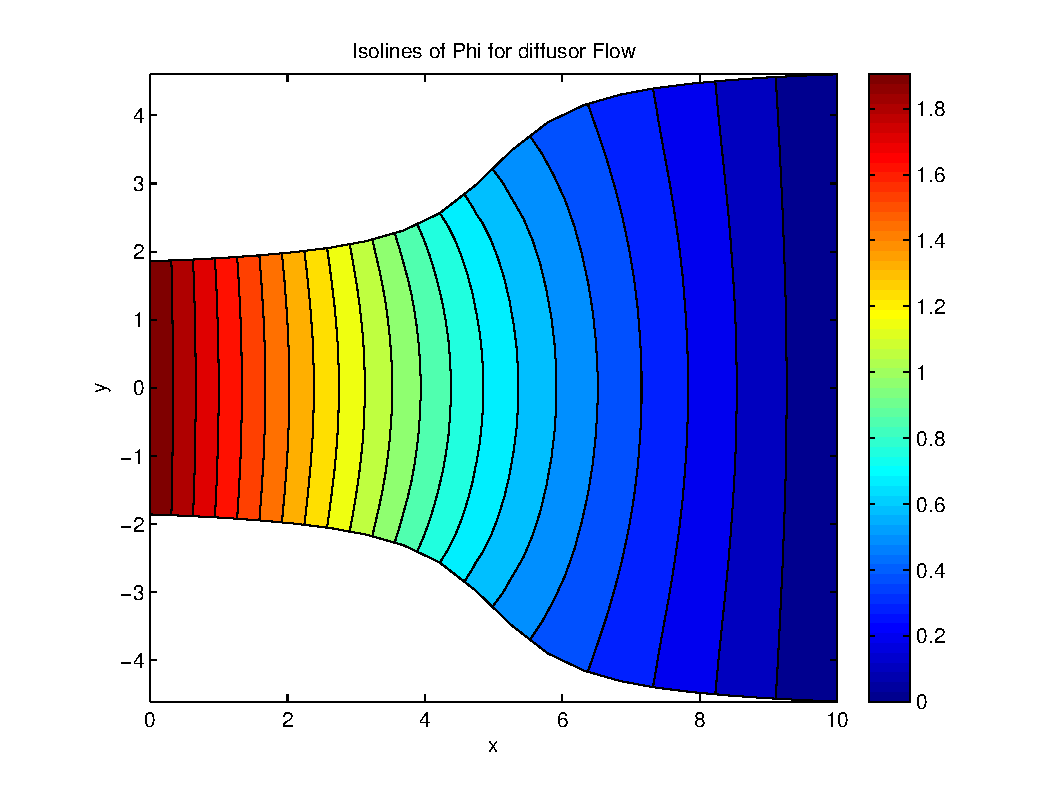
\includegraphics[scale=0.4]{test/3diffusor/phi.eps}
\includegraphics[scale=0.4]{test/3diffusor/psi.eps}\\
Hier noch einmal übereinander gelegt, so dass man erkennen kann, dass die Isolinien senkrecht aufeinander stehen. Zudem
ist auch eine Übersicht über die gegebenen Konvergenzgeschwindigkeiten bei unterschiedlichen Relaxationsfaktoren gegeben.\\
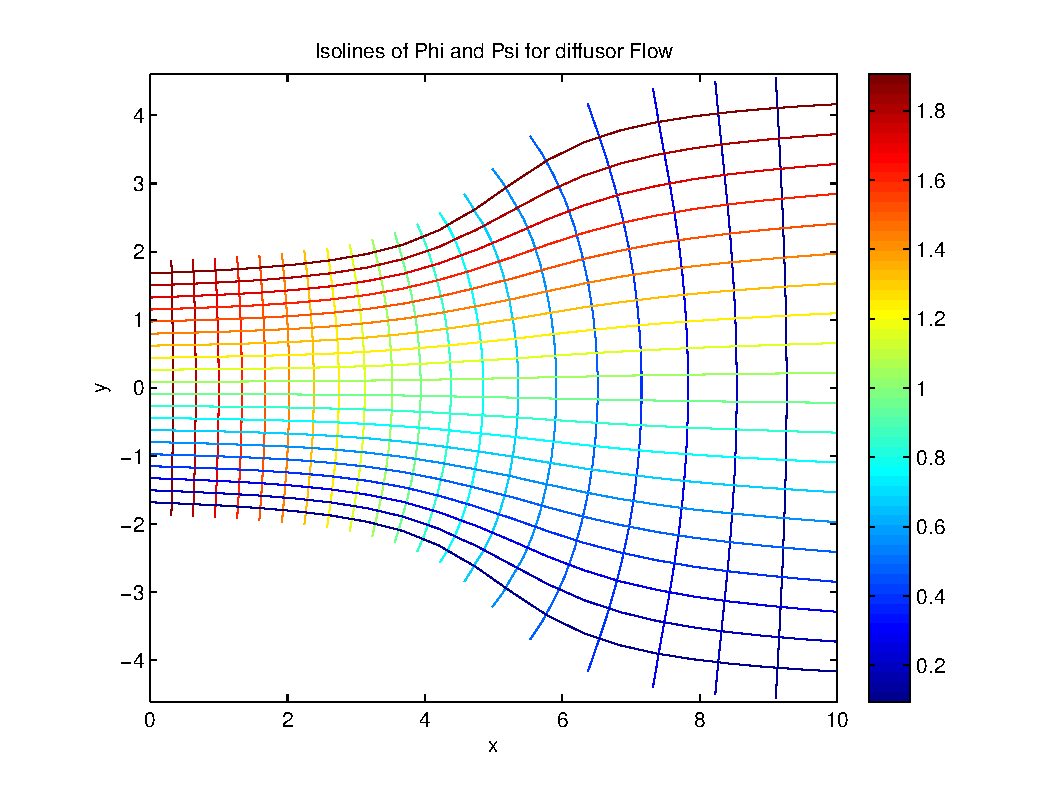
\includegraphics[scale=0.4]{test/3diffusor/both.eps}
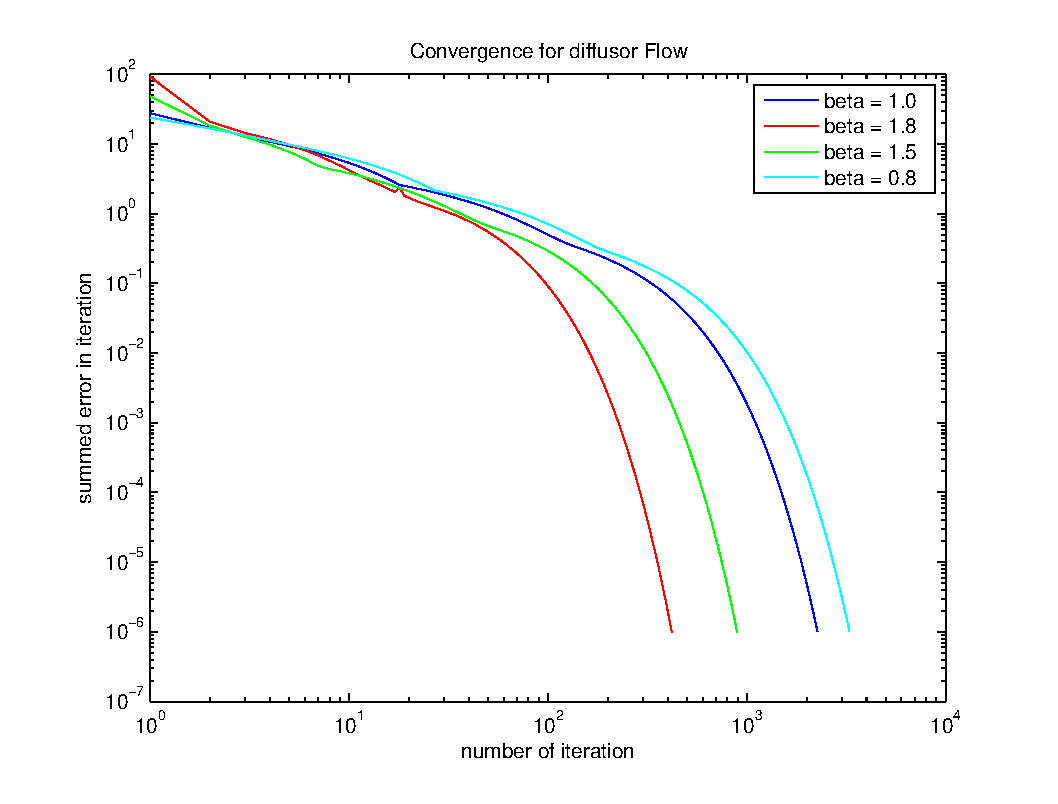
\includegraphics[scale=0.4]{test/3diffusor/error.eps}

\section{Gittergenerierung}
Die folgende Konvektions-Diffusions Strömung benötigt zur Berechnung eine Aufteilung des Gebietes in Finite Elemente.
Unser Gittergenerator unterteilt das rechteckige Gebiet in eine wählbare Anzahl an Zellen. Jede Zelle hat eine ID und ist 
umrandet von vier Kanten; Norden, Süden, Osten und Westen, welche auch nummeriert sind. So lässt sich der Fluss über den Rand
einer Zelle durch den Fluss über diese vier Kanten beschreiben.
Im folgenden ist ein Beispiele eines Gitters zu sehen. Im diesem Fall wurde das Gebiet in 3x3 Teilgebiete unterteilt.\\
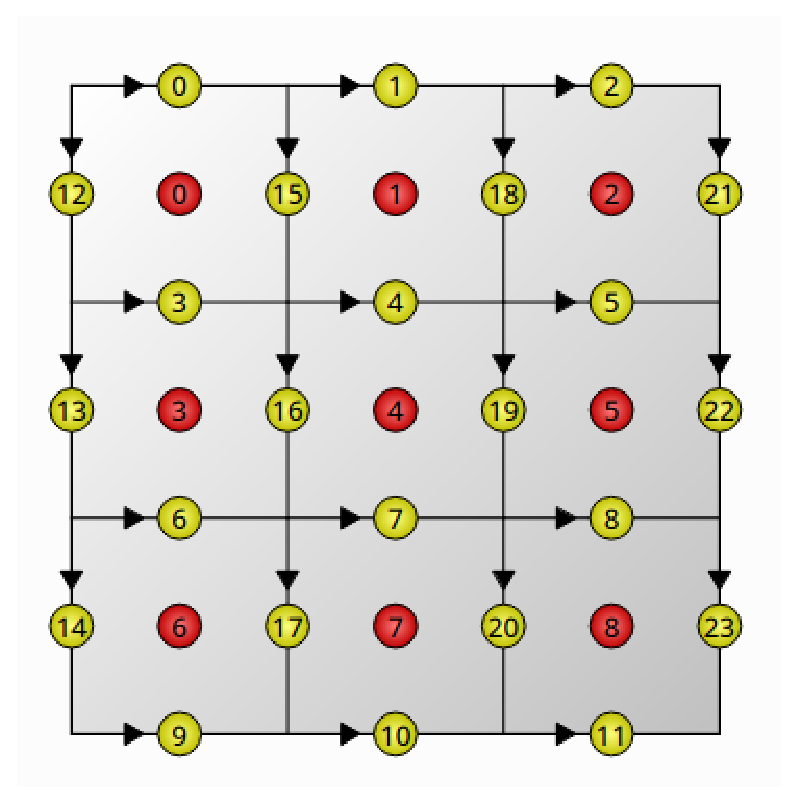
\includegraphics[scale=0.5]{test/4grid/1.eps}
%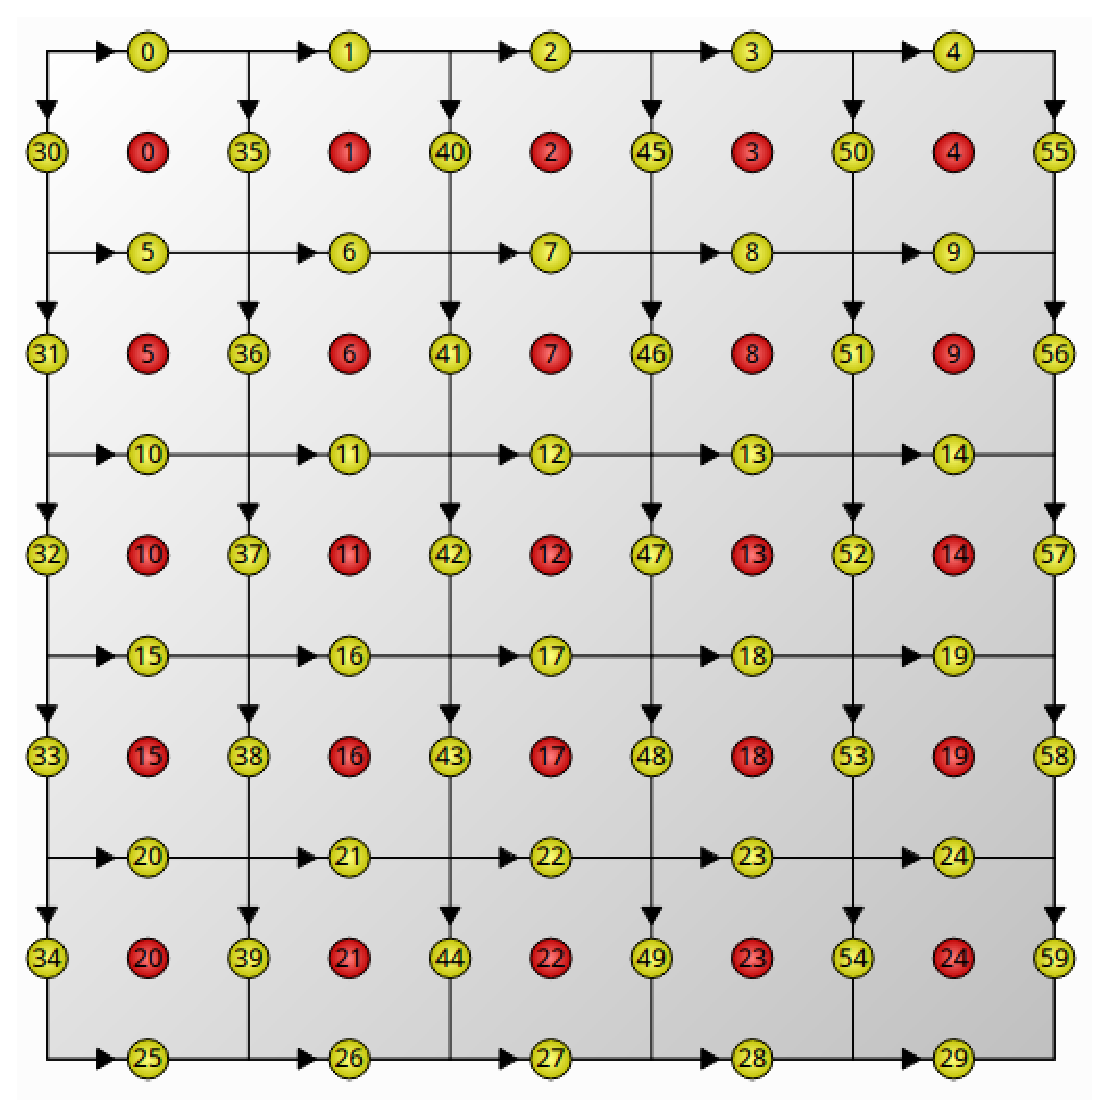
\includegraphics[scale=0.4]{test/4grid/2.eps}

\section{Konvektions-Diffusions Strömung}
Im Gegensatz zur Potentialströmung wird nun eine Strömung mittels der Finite-Elemente Methode (FEM) beschrieben. Ausgangspunkt
für die Beschreibung der Strömung ist die integrierte Kontinuitätsgleichung
\begin{align}
\ddt \int_{\Omega} \rho dV + \int_{\Omega} div(\rho v) dV = 0
\end{align}
Welche unter Anwendung des Gaußschen Integralsatzes auf folgende Form führt:
\begin{align}
\ddt \int_{\Omega} \rho dV + \oint_{\partial \Omega} (\rho v)\cdot dA = 0
\end{align}	
Zur Lösung wird im folgenden konstante Dichte $\rho$ angenommen. 
Soll auch noch Konvektion beschrieben werden, lässt sich die Erhaltungsgleichung formulieren als:
\begin{align}
\rho \int_{\Omega}\ddt \phi dV + \int_{\partial \Omega}\rho u \phi -\lambda \ddx \phi + \rho v \phi - \lambda \ddy \phi \ dA =0 
\end{align}
Diese Gleichung wird dann als Ausgangspunkt für die Diskretisierung genommen, 
da sie die Änderung des Skalars $\phi$ in abhängigkeit des Flusses über die Grenzen beschreibt.

\subsection{Diskretisierung}
Die naive Herangehensweise zur Approximierung der Strömung führt zu der Vormu
Wir approximieren das Integrationsgebiet durch rechteckige Finite Elemente, so dass der Rand des Gebietes aufgeteilt wird in vier Kanten
die im folgenden mit Norden, Osten, Süden und Westen bezeichnet werden. 
Die Änderung von $\phi$ lässt sich dann wie folgt ausdrücken:
\begin{align}
\frac{\phi^{k+1}-\phi^k}{\Delta t} = \sum_{i} f_i\cdot l_i
\end{align}
Wobei $\l_i = \Delta y$ für $i=$Westen, Osten und $\l_i = \Delta x$ für $i=$Norden, Süden.
Mit dem Fluss
\begin{align}
f_{\text{Ost}} = -(\rho u \phi_{\text{Ost}}- \lambda \ddx \phi_{\text{Ost}}), \ \ 
f_{\text{West}} = \rho u \phi_{\text{West}}- \lambda \ddx \phi_{\text{West}} \\
f_{\text{Nord}} = -(\rho v \phi_{\text{Nord}}- \lambda \ddy \phi_{\text{Nord}}),\ \ 
f_{\text{Süd}} = \rho v \phi_{\text{Süd}}- \lambda \ddy \phi_{\text{Süd}}
\end{align} 
Da unser vorgegebener Fluss aus Richtung Süd-West einströmt, verwenden wir für $\ddx \phi$ und $\ddy \phi$ das Upwind-Schema,
also $\ddx \phi \approx \frac{1}{\Delta x}(\phi_{i,j}-\phi_{i-1,j})$ und  $\ddy \phi \approx \frac{1}{\Delta y}(\phi_{i,j}-\phi_{i,j-1})$.
 
\subsubsection{Testfall nur Diffusion}
Die folgenden Testfälle sind alle auf dem selben Gitter der Dimension 20x10 gerechnet worden.
Zuerst setzten wir  $u=0$ und $v=0$ um ausschließlich Diffusion zu simulieren. Wir wählen $\lambda=0.1$ und so stellt
sich in der Theore ein lineares Profil für $\phi$ zwischen dem linken und rechten Rand ein.
Dies zeigt sich auch in unserer Berechnung. \\
\includegraphics[scale=0.4]{test/5conv/diffusiononly.eps}
 

\subsubsection{Testfall nur Konvektion}
Um zu testen, ob auch die Konvektion korrekt simuliert wird, setzen wir im folgenden $u=1$, $v=0$ und $\lambda=0$
Es ist zu erwarten, dass der Potentialwert von links über das Gitter getragen wird und sich ein nicht lineares Gefälle hin 
zum rechten Rand einstellt. Bei kurzer Simulationsdauer wird der Wert des linken Randes weniger weit in das Gebiet hineingetragen.
Lässt man $t \rightarrow \infty$, so würde sich im ganzen Gebiet der Wert des linken Randes einstellen. 
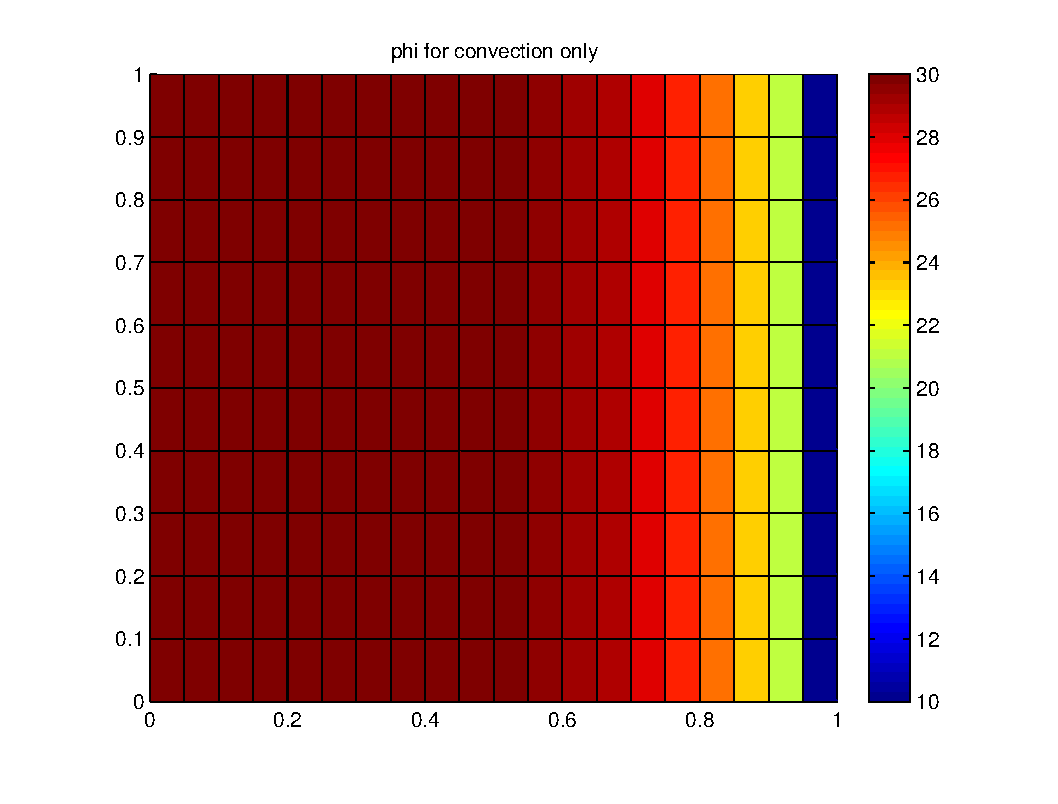
\includegraphics[scale=0.4]{test/5conv/convonly.eps}


\subsubsection{Testfall Diffusion und Konvektion a)}
Führt man nun beide Effekte zusammen so wirken die beiden Phänomen einander entgegen. So trägt die Konvektion das Potential des
Einströmrandes in das Rechengebiet, die Diffusion wirkt dem entgegen, indem sie für einen Ausgleich der Potentiale
zwischen Ein- und Auströmrand sorgt. Bei gleicher Geschwindigkeit bewirkt ein größeres $\lambda$, dass die Lösung des linken Randes weniger weit
in das Rechengebiet eindringt. Die beiden Grafiken zeigen dieses Phänomen für $\lambda=0.2$ und $\lambda = 0.9$.\\
\includegraphics[scale=0.4]{test/5conv/alpha0.2.eps}
\includegraphics[scale=0.4]{test/5conv/alpha0.9.eps}

\subsubsection{Testfall Diffusion und Konvektion b)}
Zuletzt wollen wir den Fall simulieren, dass $u=v=1$ und $\lambda>0$ gilt. Das heißt, dass unsere Strömung aus Richtung Süd-West in das Rechengebiet
einströmt. Da oberer und unterer Rand eine undurchlässige Wand darstellen, bewirkt die Konvektion, dass sich am oberen linken Rand das höchste Potential einstellt, da sich 
an dieser Stelle ein Staupunkt der Strömung befindet. Somit steigt das Potential an diesem Staupunkt für längere Simulationsdauer immer weiter an, bis sich ein
stationärer Wert einstellt, in dem die Diffusion das Ansteigen des Potentials durch die Konvektion kompensiert. Das Rechengbiet
wurde in diesem Fall in 30x30 Zellen aufgeteilt.\\
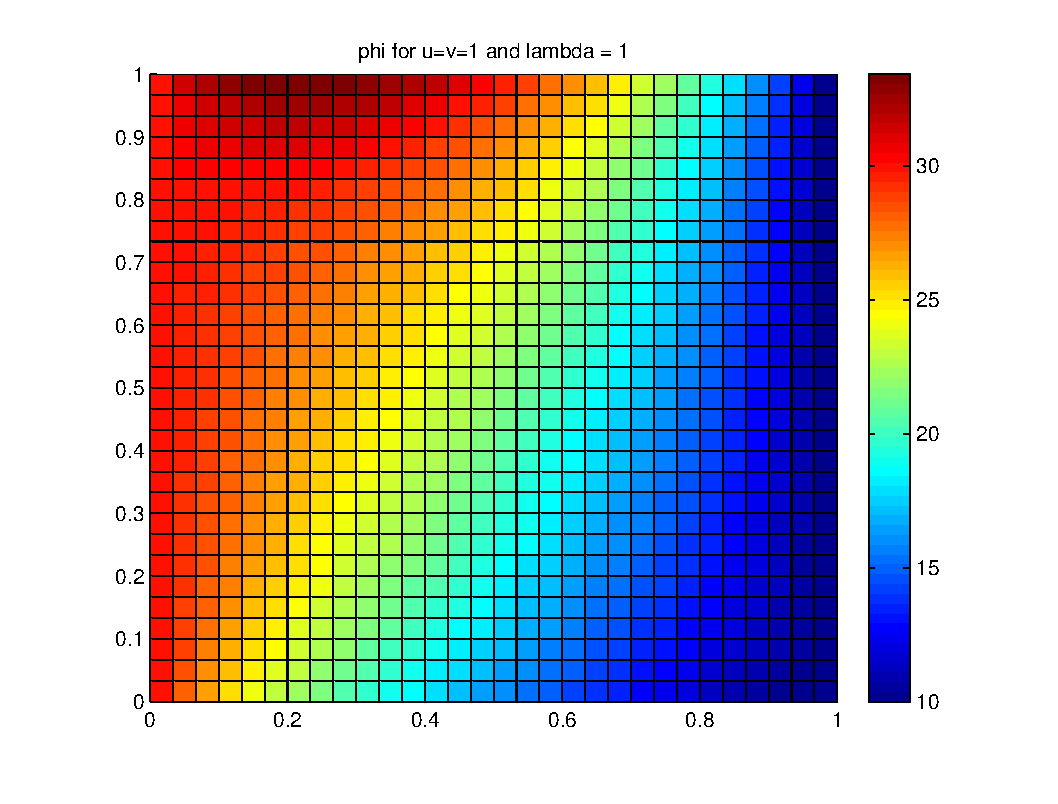
\includegraphics[scale=0.6]{test/5conv/uvl.eps}

\subsection{Analytische Lösung }
Für den Fall einer eindimensionalen Strömung lässt sich
 mittels der Peclet Zahl $Pe = \frac{\rho u l }{\lambda}$ eine analytische Lösung angeben
 Man kann eine  Iterationsvorschrift für $\phi_{i,j}$ in Abhängigkeit der Peclet Zahl aufstellen. 
 Das Verfahren ist damit für den instationären Fall gegeben als:
 \begin{align}
 \tilde{a}_p \phi^{\nu+1} &= a_o \phi_o+a_w \phi_w+ + a_n \phi_n+a_s\phi_s + b \\
 b &= \rho \frac{\Delta x \Delta y}{  \Delta t}\phi_p^{\nu} \\
 \tilde{a}_p &= a_o + a_w+a_n+a_s + \rho \frac{\Delta x \Delta y}{  \Delta t}
 \end{align}
wobei sich die Koeffizienten $a_{o,n,w,s}$ in Abhängigkeit der Peclet Zahl schreiben lassen.
\begin{align*}
a_{o} &= D_{o} \Delta y A(|Pe_{o}|) + \max (-f_{o} \Delta y , 0)\\
a_{o} &= D_{w} \Delta y A(|Pe_{w}|) + \max (f_{w} \Delta y , 0)\\
a_{s} &= D_{s} \Delta x A(|Pe_{s}|) + \max (f_{s} \Delta x , 0)\\
a_{n} &= D_{n} \Delta x A(|Pe_{n}|) + \max (-f_{n} \Delta x , 0)
\end{align*}
Die Koeffizienten $D_{o,w,s,n}$ liefern eine Reihe von Verfahren. Hier seien nur kurz das Exponentialgesetzt
Zentral Differenzen und das Upwind Verfahren 1. Ordnung erwähnt.

\subsection{Lösung der Impulsgleichung}
Setzt man nun nicht mehr das Geschwindigkeitsfeld als gegeben vorraus, lässt sich dieses
mit Hilfe der Impulsgleichungen aus dem Druckfeld bestimmen:
\begin{align}
\ddt(\rho u) +\ddx\phi_x = -\ddx p \\
\ddt(\rho v) +\ddy\phi_y = -\ddy p 
\end{align}
mit 
\begin{align}
\phi_x = \rho u u - \eta \ddx u\\
\phi_y = \rho v v - \eta \ddy v
\end{align}
Aus diesen Gleichungen lässt sich das Geschwindigkeitsfeld in direkter Abhängigkeit zum Druckfeld lösen.
Da die Impulsgleichungen die selbe Struktur haben wie die Konvektions-Diffusions Gleichungen lässt sich
das Geschwindigkeitsfeld mit einem ähnlichen Ansatz lösen.
\begin{align}
\tilde{a}_p u_e^{\nu+1}= a_o u^{\nu}_o+a_w u^{\nu}_w +a_n u^{\nu}_n +a_s u^{\nu}_s +b +(p_p-p_E)\Delta y_P\\
\tilde{a}_p v_e^{\nu+1}= a_o v^{\nu}_o+a_w v^{\nu}_w +a_n v^{\nu}_n +a_s v^{\nu}_s +b +(p_p-p_E)\Delta x_p
\end{align}
Mit den gleichen Koeffizienten wie in (22).
Wir setzen den Druck als gesuchten Wert in der Zelle an und betrachten die Geschwindigkeiten
auf den Zellrändern. Ein Problem welches bei der Diskretisierung mittels finiter DIfferenzen entsteht
ist eine Entkopplung benachbarter Drücke. Somit kann es zu einem hohen Druckgradienten zwischen den Stellen
$(i,j)$ und $(i+1,j)$ kommen, dieser würde aber unberücksichtigt bleiben, da der Druckgradient
zwischen $(i,j)$ und $(i+2,j)$  gleich null ist. Das Resultat wäre eine Zick-Zack-Verteilung des Druckes. Deshalb werden im folgenden versetzte Gitter benutzt, welche das Problem
der Entkopplung vermeiden.\\

\subsection{Testfälle der Impulsgleichung}
Wir testen den Ansatz mit Hilfe der Couette Strömung.
//Le Bilder







\end{document}